%==============================================================
%Encap�alament
%==============================================================
\documentclass[a4paper,oneside,12pt]{article}
\usepackage[left=2.5cm,right=2cm,top=2cm,bottom=2cm]{geometry}
\usepackage[catalan]{babel}
\usepackage[T1]{fontenc}
\usepackage[latin1]{inputenc}
\usepackage{graphicx} % Required for including pictures
\usepackage{subfigure} % subfiguras
\usepackage{float} % Allows putting an [H] in \begin{figure} to specify the exact location of the figure
\usepackage{wrapfig} % Allows in-line images
\linespread{1.2}
\graphicspath{{Pictures/}}

\usepackage{subscript} %super�ndexs i sub�ndexs
\setcounter{secnumdepth}{5} %Numerar fins a subpar�grafs
\usepackage{pdfpages} %posar arxius pdf (com articles...)

\usepackage{amssymb, amsmath, amsbsy} % librerias ams
\usepackage{stackrel} %Escriure a sobre o sota de qualsevol fletxa
\usepackage{color}
\usepackage{multicol}
\usepackage{array}
\usepackage[full]{textcomp}
\usepackage{multirow}

% Enumeracions
\usepackage[shortlabels]{enumitem}
\usepackage{pstricks}

\usepackage{tikz}
\newcommand*{\itembolasazules}[1]{% bolas 3D 
	\footnotesize\protect\tikz[baseline=-3pt]% 
	\protect\node[scale=.7, circle, shade, ball
	color=blue]{\color{white}\Large\bf#1};}

\newcommand*{\itembolasverdes}[1]{% bolas 3D 
	\footnotesize\protect\tikz[baseline=-3pt]% 
	\protect\node[scale=.7, circle, shade, ball
	color=green]{\color{white}\Large\bf#1};}

\newcommand*{\itembolasrojas}[1]{% bolas 3D 
	\footnotesize\protect\tikz[baseline=-3pt]% 
	\protect\node[scale=.7, circle, shade, ball
	color=red]{\color{white}\Large\bf#1};}

% Lletres gregues
\DeclareRobustCommand{\greektext}{%
  \fontencoding{LGR}\selectfont\def\encodingdefault{LGR}}
\DeclareRobustCommand{\textgreek}[1]{\leavevmode{\greektext #1}}
\DeclareFontEncoding{LGR}{}{}
\DeclareTextSymbol{\~}{LGR}{126}

%Bibliografia
\usepackage[square]{natbib}

% Instruccions especials
\newcommand{\seny}{senyalitzaci�}
\newcommand{\aas}{amino�cids}
\newcommand{\TF}{factor de transcripci�}
\newcommand{\TFs}{factors de transcripci�}
\newcommand{\tgfb}{TGF\textgreek{b}}
\newcommand{\pparg}{PPAR\textgreek{g}}
\newcommand{\betaadren}{\textgreek{b}-adren�rgic}
\newcommand{\Rbeta}{R\textsubscript{\textgreek{b}}}
\newcommand{\iso}{isoproterenol}
\newcommand{\aden}{adenilat ciclasa}
\newcommand{\ca}{Ca\textsuperscript{2+}}
\newcommand{\betacat}{\textgreek{b}-catenina}
\newcommand{\fletsup}{$\uparrow$}
\newcommand{\fletinf}{$\downarrow$}
\newcommand{\gng}{gluconeog�nesi}
\newcommand{\tnfa}{TNF-\textgreek{a}}
\newcommand{\ikb}{I\textgreek{k}B\textgreek{a}}
\newcommand{\nfkb}{NF-\textgreek{k}B}
\newcommand{\pgc}{PGC-1\textgreek{a}}
\newcommand{\na}{Na\textsuperscript{+}}
\newcommand{\pot}{K\textsuperscript{+}}
\newcommand{\ags}{�cids grassos}
\newcommand{\ck}{cicle de Krebs}
\newcommand{\ag}{�cid gras}
\newcommand{\ppara}{PPAR\textgreek{a}}
\newcommand{\ppard}{PPAR\textgreek{d}}
\newcommand{\ifng}{IFN-\textgreek{g}}

% F�rmules qu�miques
\usepackage{chemformula}
%\usepackage[version=4,arrows=pgf]{mhchem}
\usepackage{texshade}
\usepackage{textopo}

%\newcommand{\powd}[1]{$10^{#1}$}
%\newenvironment{?}{?}{?}

\setcounter{tocdepth}{2} % numerar fins subseccions a TOC

% Encap�alament i peu de p�gina
\usepackage{fancyhdr}
\pagestyle{fancy}
%\renewcommand{\sectionmark}[1]{\markright{\textsc{\thesection. #1}}}
\lhead{}
\rhead{}
\lfoot{\sc Bioqu�mica Anal�tica i Cl�nica}
%\rfoot{\thepage}
\cfoot{}

\fancyfoot[R]{\thepage}

\renewcommand{\headrulewidth}{0.4pt}
\renewcommand{\footrulewidth}{0.4pt}

\raggedbottom
\providecommand{\tabularnewline}{\\}


% Format seccions
%\usepackage{sectsty}
%\sectionfont{\centering\nohang\LARGE\bfseries}
%\partfont{\centering\huge\red}
\usepackage{titlesec}

\titleformat{\section}[block]{\centering}{\bfseries\LARGE\thesection  . }{0em}{\LARGE\bfseries}{}

\titleformat{\subsection}[hang]{\flushleft}{\bfseries\Large\thesubsection }{0.2cm}{\Large\bfseries}

\titleformat{\subsubsection}[hang]{\flushleft}{\bfseries\large\thesubsubsection }{0.2cm}{\large\bfseries}

% Format parts
%\titleformat{\part}[hang]{\centering\vspace{-1.75cm}}{\bfseries\huge\thepart . }{0em}{\huge \bfseries}{}
\newcommand{\titline}{\titlerule[2pt]}
\titleformat{\part}[hang]
  {\vspace{-2cm}\sc\bfseries\huge\red}{\centering\huge\sc\bfseries
  	}
  {0ex}
  {\titline \\
   \vspace{1pt}%
   \centering\huge\sc\bfseries\red\thepart . }
   [%
 \titline]

\usepackage[hyperindex,linktocpage]{hyperref}

% Format �ndex
\usepackage{kpfonts}
\usepackage{titletoc}
\contentsmargin{0cm}
\titlecontents{part}[0pc]
{\addvspace{30pt}%
	\\\color{red}\large\sc\bfseries}%
{}
{}
{\;\titlerule\;\large\bfseries \thecontentspage}%
\titlecontents{section}[2.4pc]
{\addvspace{1pt}}
{\bfseries\contentslabel[\thecontentslabel]{2.4pc}}
{}
{\hfill\small\bfseries\thecontentspage}
[]
\titlecontents*{subsection}[4pc]
{\addvspace{-1pt}\small}
{}
{}
{\ --- \small\thecontentspage}
[ \textbullet\ ][]
%%--


% ====================ENTORNS ====================
\usepackage{tikz,tkz-tab}
\usepackage{tcolorbox, empheq}%

% Entorn per dades
\definecolor{colordadesfons}{RGB}{255,255,255}
\definecolor{colordadesmarc}{RGB}{108, 217, 0}

%\definecolor{colorrecfons}{RGB}{203,216,227}
\definecolor{colorrecfons}{RGB}{255,255,255}
\definecolor{colorrecmarc}{RGB}{128,177,221}

\tcbuselibrary{theorems}
\newtcbtheorem[number within=section]{dades}{An�lisi de dades} {colback=colordadesfons,colframe=colordadesmarc,fonttitle=\bfseries,separator sign={\ $\blacktriangleright$}}{theo}

\newtcbtheorem[number within=section]{rec}{Recordatori} {before=\begin{center},after=\end{center},colback=colorrecfons,colframe=colorrecmarc,fonttitle=\bfseries,separator sign={\ $\blacktriangleright$}}{theo}

\newtcbtheorem[number within=section]{metodes}{M�todes} {colback=red!5!white,colframe=red!75!black,fonttitle=\bfseries,separator sign={\ $\blacktriangleright$}}{theo}

% Equacions
\tcbuselibrary{skins,breakable}
\newcounter{example}
\colorlet{colexam}{red!75!black}

\newtcolorbox[]{myexample}[2][]{%
	empty,title={#1 \thetcbcounter},attach boxed title to top left,
	boxed title style={empty,size=minimal,toprule=2pt,top=4pt,
		overlay={\draw[colexam,line width=2pt]
			([yshift=-1pt]frame.north west)--([yshift=-1pt]frame.north east);}},
	coltitle=colexam,fonttitle=\Large\bfseries,
	before=\par\medskip\noindent,parbox=false,boxsep=0pt,left=0pt,right=3mm,top=4pt,
	breakable,pad at break*=0mm,vfill before first,
	overlay unbroken={\draw[colexam,line width=1pt]
		([yshift=-1pt]title.north east)--([xshift=-0.5pt,yshift=-1pt]title.north-|frame.east)
		--([xshift=-0.5pt]frame.south east)--(frame.south west); },
	overlay first={\draw[colexam,line width=1pt]
		([yshift=-1pt]title.north east)--([xshift=-0.5pt,yshift=-1pt]title.north-|frame.east)
		--([xshift=-0.5pt]frame.south east); },
	overlay middle={\draw[colexam,line width=1pt] ([xshift=-0.5pt]frame.north east)
		--([xshift=-0.5pt]frame.south east); },
	overlay last={\draw[colexam,line width=1pt] ([xshift=-0.5pt]frame.north east)
		--([xshift=-0.5pt]frame.south east)--(frame.south west);},% 
}

\begin{document}

%----------------------------------------------------------
%Portada
%----------------------------------------------------------
\begin{titlepage}

\newcommand{\HRule}{\rule{\linewidth}{0.5mm}} % Defines a new command for the horizontal lines, change thickness here

\center % Center everything on the page
\HRule \\[0.4cm]
{\Huge\bfseries\textsc{Bioqu�mica Anal�tica i Cl�nica}} \\[0.4cm] % Title of your document
\HRule \\[04cm]
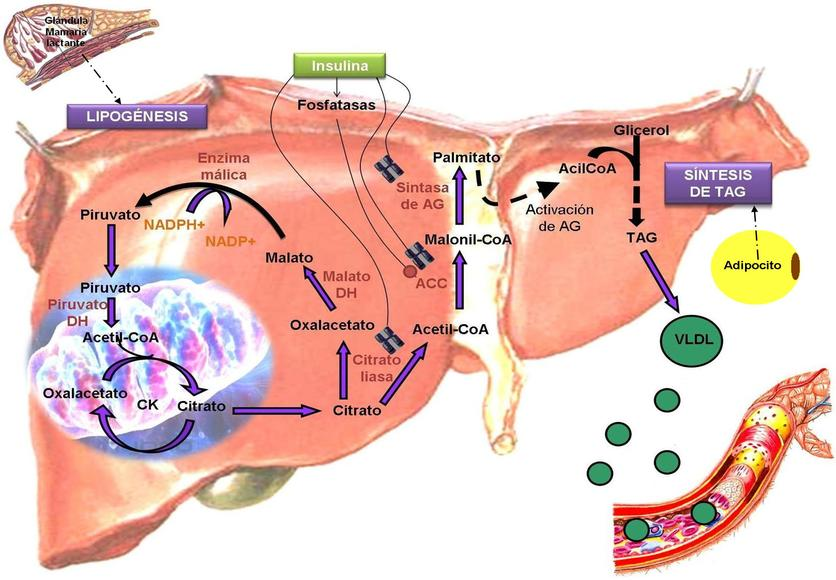
\includegraphics[width=1\textwidth]{Logo} %Include a department/university logo

\vspace{1cm}
\textsc{\Large Ci�ncies Biom�diques UB - Primavera 2017}\\[0.5cm] % Minor heading such as course title
\vspace{0.5cm}
\textsc{\large Albert Torell� P�rez}
\vfill % Fill the rest of the page with whitespace
\end{titlepage}

%===================================
\renewcommand{\figurename}{\textsc{{Figura}}}
\renewcommand{\tablename}{\textsc{{Taula}}}
\renewcommand{\thefootnote}{\alph{footnote}}

%------------------------------------------------------------------------------
%Cos dels apunts 
%------------------------------------------------------------------------------
\pagenumbering{Roman} % para comenzar la numeraci�n de paginas en n�meros romanos

%----------------------------
% Taula de continguts
%----------------------------
\tableofcontents

\pagenumbering{arabic}
%------------------------------------------------------------------------------
% Tema 1. Variabilitat Cl�nica
%------------------------------------------------------------------------------
\newpage
%------------------------------------------------------------------------------
% Tema 1. Embrionic Stem Cells
%------------------------------------------------------------------------------
\section{\textit{Embrionic Stem Cells}}
D'una cèl·lula embrionària és interessant obtenir-ne clons. Dels diferents clons que s'obtenen s'ha de comprovar la pluripotencialitat.

Una \textbf{stem cell} és una cèl·lula que presenta 2 propietats (poden ser endògenes o induïdes):
\begin{enumerate}
\item Auto-renovació: es pot dividir de manera que s'obté una cèl·lula idèntica. P.e els fibroblasts presenten aquesta característica. La divisió és simètrica. La capacitat d'auto-renovació depèn de cada clon. El grau d'auto-renovació d'una ESC és dels més alts que es poden aconseguir, en canvi una cèl·lula del mesoderma ja té una capacitat d'auto-renovació més limitada. Una ESC es pot mantenir 1 any \textit{in vitro}. Les cèl·lules mare adultes han perdut la capacitat d'autorenovació.

\item Capacitat de diferenciació: Capacitat de generar una cèl·lula especialitzada per divisió asimètrica (morfologia, patró epigenètic, destí cel·lular). Molts medis de cultiu per cèl·lules mare bloquegen la capacitat de diferenciació.
\end{enumerate}

\subsection{Blastocist pre-implantacional}
Aquest blastocist no està adherit a l'úter, ja que quan s'adhereix a l'úter pateix canvis de morfologia, llinatges, importants. És aproximadament als 5 dies de gestació. S'obtenen cèl·lules de l'estadu entre massa interna i la generació dels 3 fulls embrionaris. Si la massa interna es deixa desenvolupar, es comença a diferenciar. Es força a que la massa interna sigui una \textit{stem cell}.

No totes les ESC són capaces de generar cèl·lules de línia germinal.

Hi ha diferents graus de potència:
\begin{description}
\item[Totipotents] Són els zigots. Poden donar lloc a un organisme sencer ben format. Té una capacitat proliferativa il·limitada i pot desenvolupar tots els teixits i òrgans post-embrionaris

\item[Pluripotents] Són les ESC, del blastocist... Tenen la capacitat d'originar varietats de tipus cel·lulars i teixits.

\item[Multipotents] P.e les cèl·lules mesenquimals. Especialitzades en originar únicament determinats tipus cel·lulars de determinats teixits.
\end{description}

Les \textit{germinal stem cells} també tenen potència. Les iPSC són cèl·lules adultes que s'han desdiferenciat artificialment amb un alt grau de potència.

Les cèl·lules de la medul·la òssia són cèl·lules mesenquimals i hematopoiètiques.

Temple, Nature Reviews Neuroscience, 2005

\subsubsection{Experiments quimera}
Tenen per objectiu demostrar si les cèl·lules són pluripotents o no.

S'obtenen 2 tipus cel·lulars d'un animal que expressa constitutivament la fosfatasa alcalina. Després s'injecten en un blastocist pre-implantacional i es col·loquen en una mare receptora (el grau d'implantació és molt petit). Es recullen els embrions a E11 i es revela l'activitat fosfatasa alcalina.

Si tots els teixits presenten coloració, estem parlant que les cèl·lules injectades són embrionàries.
Si no tots els teixits presenten coloració, vol dir que la potència d'aquestes cèl·lules és més limitada.

En ESC, el control de la divisió cel·lular és molt complicat.

\subsection{Obtenció de cèl·lules mare}
Es poden obtenir per 3 procediments:
\begin{enumerate}
\item Aïllament de la massa cel·lular interna
\item Aïllament de cèl·lules primmordials de l'embrió
\item Transferència nuclear a partir de cèl·lules somàtiques adultes
\end{enumerate}

Aquestes tècniques han evolucionat en paral·lel a FIV.

Un teratoma és un tumor sòlid que conté cèl·lules proliferatives de les 3 capes embrionaries. Per generar els teratomes, s'injectaven les cèl·lules a escrot de ratolí o subdèrmic. Les iPSC tenen la capacitat de produir teratomes.

Quan s'aïlla la massa interna, no s'obté de manera pura. El cultiu pretén recrear les condicions del blastocist. Si són humanes, es plaquegen sobre una capa de fibroblasts irradiats que donen suport físic i biològic (factors de creixement, citocines). El fibroblasts són de prepuci de ratolí, són línies establertes que aguanten molt bé la irradiació. Passats uns dies, es forma un cos embrioide. S'agafen cèl·lules de la perifèria, les cèl·lules del centre estan en hipòxia i les cèl·lules del voltant es diferencien per l'acció del ROS. Aquestes cèl·lules de la perifèria es passen a una altra placa i així successivament fins que s'obtenen clons de ESC.

En el ratolí, hi ha un punt que no es requereix la capa de fibroblasts.

%------------------------------------------------------------------------------
% Tema 2. Semiologia
%------------------------------------------------------------------------------
\newpage
%------------------------------------------------------------------------------
% Tema 2. Semiologia
%------------------------------------------------------------------------------
\section{Semiologia}

\subsection{Valors de referència}
La població de referència és la població individus sans (normals). Per estudiar-ho, s'agafa una mostra de referència, que és un nombre assequible i representatiu de la població de referència.

\begin{description}
\item[Valors de referència] Rang de resultat analític de la determinació d'un paràmetre bioquímic en espècimens d'individus de referència.

\item[Capacitat discriminant] Propietat de donar valors diferents en individus d'una població normal ($\hat{E}$) respecte els d'una població patològica (E).
\end{description}

%------------------------------------------------------------------------------
% Tema 3.
%------------------------------------------------------------------------------
%\newpage
%%------------------------------------------------------------------------------
% Tema 3. Control de qualitat
%------------------------------------------------------------------------------
\section{Control de qualitat}
\label{sec:control-de-qualitat}

La garantia de qualitat es fa a diversos nivells.

Els valors donats han de ser precisos i exactes.



%------------------------------------------------------------------------------
% Tema 4. Prote�nes plasm�tiques
%------------------------------------------------------------------------------
\newpage
%-------------------------------------------------------------------------------
% Tema 4. Malalties del genoma mitocondrial
%-------------------------------------------------------------------------------
\section{Malalties del genoma mitocondrial}
\label{sec:mitocondrial}

Els conceptes de domin�ncia i recessivitat no s'apliquen exactament aqu�.

Les malalties del DNA mitocondrial no es consideren diagnosticades fins que es fa el diagn�stic molecular/gen�tic.

\subsection{Biologia del DNA mitocondrial}
\label{sec:dnamitocondrial}

El DNA mitocondrial representa l'1\% del DNA cel�lular total en funci� del nombre de mitocondris de la c�l�lula.

El DNA mitocondrial �s circular de doble cadena i de 16,7 kb. S'assumeix que tots els mitocondris tenen DNA mitocondrial.S'assumeix que hi ha poques c�pies del DNA mitocondrial, entre 3 i 4 per mitocondri i entre 1000 i 10000 c�pies per c�l�lula.. Els gens del genoma mitocondrial no tenen introns i nom�s una regi� no codificant que t� els elements reguladors comuns. Hi ha m�s c�pies de gens mitocondrials que de gens nuclears.

Cont� 13 mRNA, 22 tRNA i 2 rRNA. Els 13 mRNA codifiquen per 13 prote�nes components de la cadena respirat�ria i fosforilaci� oxidativa. % Mecanisme de cadena respirat�ria i fosforilaci� oxidativa

\begin{figure}[H]
\centering
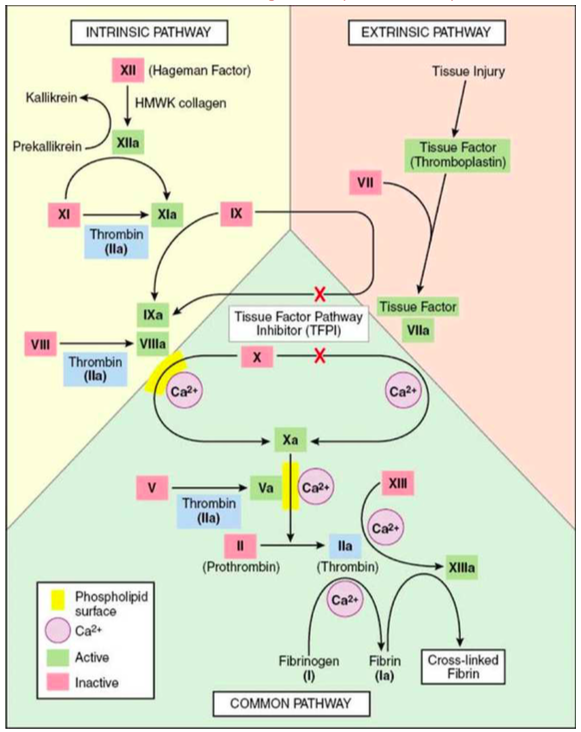
\includegraphics[width=0.8\textwidth]{fig26}
\label{fig26}
\end{figure}

Es reparteixen aix�:
\begin{itemize}
\item Complex I (NADH deshidrogenasa): 7 subunitats
\item Complex III: 1 subunitat
\item Complex IV: 3 subunitats
\item Complex V (ATP sintasa): 2 subunitats. Sense el gradient de protons, aquest enzim �s una ATPasa.
\end{itemize}

\begin{figure}[H]
\centering
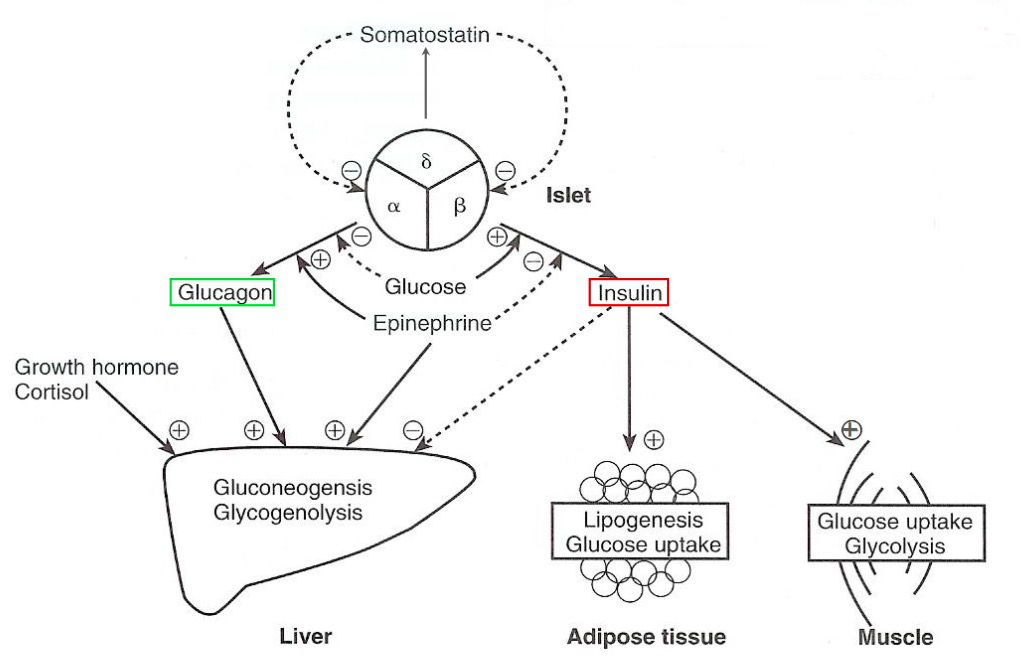
\includegraphics[width=0.6\textwidth]{fig27}
\label{fig27}
\end{figure}

El genoma mitocondrial es coordina amb el genoma nuclear per sintetitzar els complexes mitocondrials sincr�nicament. El mitocondri t� un sistema de traducci� propi. Els ribosomes mitocondrials s�n m�s petits. Els rRNA (12S i 18S) components d'aquests ribosomes estan codificats al genoma mitocondrial. Les prote�nes dels ribosomes mitocondrials estan codificats al genoma nuclear. Els tRNA s�n menys petits i diversos, amb un codi gen�tic diferent.

El D-loop �s una zona no codificant que t� els elements reguladors de la replicaci� i la transcripci�. Les 2 cadenes del genoma mitocondrial s'anomenen H i K (\textit{heavy} i \textit{light}). La que t� pocs gens �s la L i la H cont� molts gens.

El DNA mitocondrial es transcriu en bloc, d�na lloc a un mRNA policistr�nic que es processa i produeix els RNA espec�fics. Es fa un transcrit que comen�a al D-loop i despr�s continua per tota la cadena H. La transcripci� es pot aturar fins a la seq��ncia del tRNA de la Leu. La RNA polimerasa �s diferent que la del genoma nuclear.

Hi ha 2 opinions sobre la finalitzaci� prematura:
\begin{itemize}
\item Factors a l'inici de la transcripci�
\item Factors al final de la transcripci�
\end{itemize}

La replicaci� del DNA mitocondrial va desacoblada a la replicaci� del genoma nuclear. Una c�l�lula proliferativa pot no replicar el DNA mitocondrial i una c�l�lula quiescent pot replicar el DNA mitocondrial. En l'exercici cr�nic, hi ha una replicaci� de DNA mitocondrial al m�scul esquel�tic per refor�ar la cadena respirat�ria. La replicaci� del genoma mitocondrial comen�a al D-loop i es replica nom�s la cadena H fins a una zona reguladora en qu� comen�a la cadena L. Es forma un heterotr�plex: les 2 cadenes mare i un tros de la cadena nova. La DNA polimerasa �s diferent de la nuclear, est� codificada al DNA nuclear i es sintetitza al citoplasma.

\subsection{Mutacions al genoma mitocondrial}
\label{sec:mutacions-al-genoma}
La taxa de mutaci� �s m�s alta que al genoma nuclear. Aix� s'explicaria perqu� el DNA mitocondrial no est� estructurat en cromatina. Es considera que el DNA mitocondrial est� m�s exposat a mut�gens. Al mitocondri es generen moltes ROS, que s�n potents mut�gens. Si la reducci� de l'oxigen �s incompleta, es formen ions super�xid.

Les mutacions podran ser polim�rfiques o patol�giques. La primera seq��ncia que es va obtenir es fa servir de refer�ncia i s'anomena seq��ncia Cambridge. Un problema important �s discriminar la patogenicitat de la mutaci�.

\subsection{Her�ncia del genoma mitocondrial}
\label{sec:herencia-del-genoma}
El DNA mitocondrial no es recombina i �s de transmissi� materna.

La ovella Dolly es va obtenir enucleant un o�cit i introduint el nucli d'una c�l�lula som�tica. S'ent�n que una part del DNA mitocondrial es va transferir de la c�l�lula som�tica a l'o�cit. L'o�cit tindria un sistema de reconeixement i degradaci� selectiva del DNA mitocondrial exogen.

L'her�ncia de la mutaci� no ser� mendeliana. Moltes vegades s�n espont�nies per�.

\begin{figure}[H]
\centering
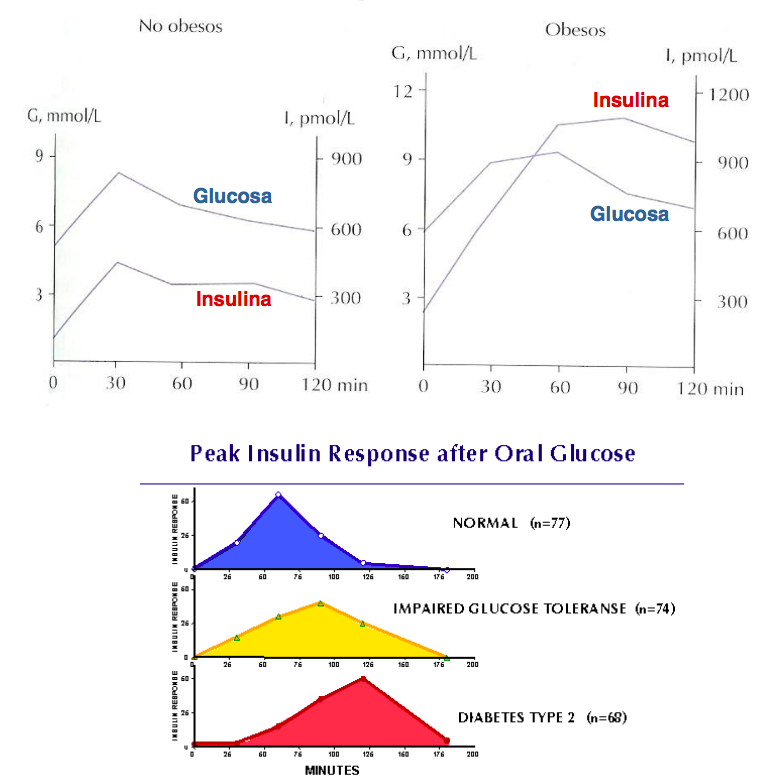
\includegraphics[width=0.8\textwidth]{fig28}
\label{fig28}
\end{figure}

En el pacient poden existir mol�cules de mtDNA sanes i mutades. Quan les seq��ncies de mtDNA s�n id�ntiques hi ha homopl�smia. Les manifestacions polim�rfiques es consideren en homopl�smia.

La heteropl�smia es d�na quan hi ha diferents mol�cules de mtDNA. Es d�na la dada en percentatge.

La heteropl�smia pot presentar difer�ncies entre germans de mare i en funci� del teixit. Les c�l�lules sangu�nies tenen menys grau d'heteropl�smia, les c�l�lules en divisi� tenen menys heteropl�smia. Les dades en sang no s�n informatives i s'ha de fer una bi�psia generalment muscular per diagnosticar la heteropl�smia a nivell molecular.

\begin{figure}[H]
\centering
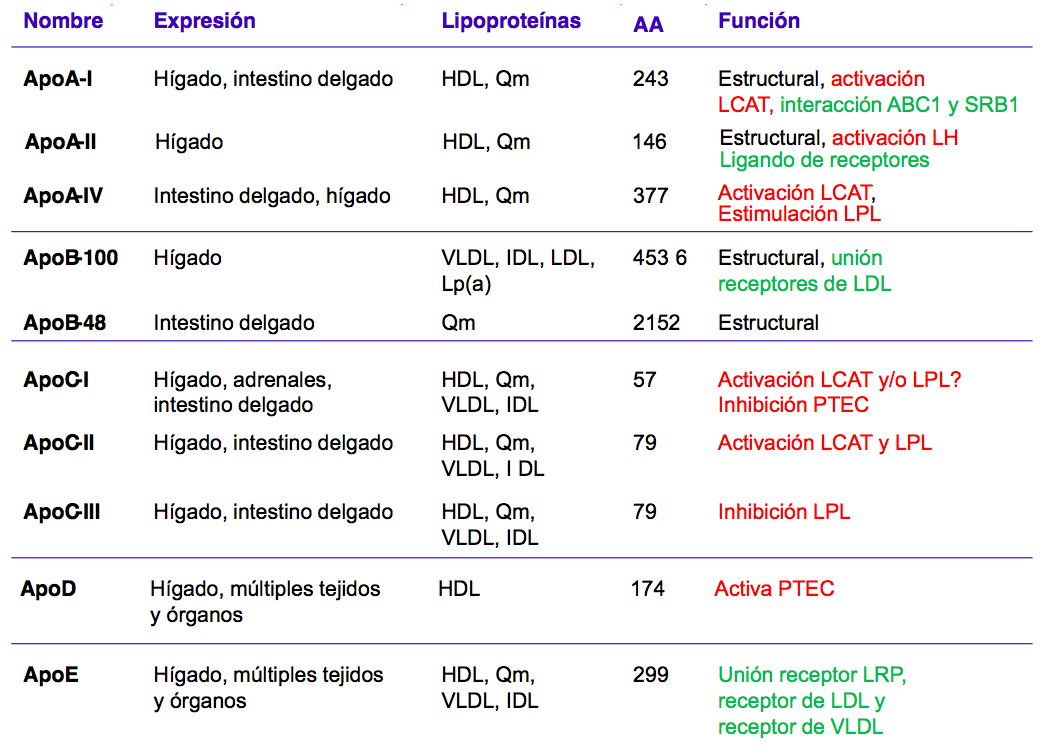
\includegraphics[width=0.8\textwidth]{fig29}
\label{fig29}
\end{figure}

Hi ha un efecte llindar en relaci� als s�mptomes. A partir de cert grau d'heteropl�smia es pot no manifestar cap s�mptoma. Com m�s heteropl�smia hi hagi, m�s greu ser� la malaltia. Amb un 30\% d'heteropl�smia no hi ha cap s�mptoma, p.e.

S�n malalties progressives que empitjoren amb l'edat. Els s�mptomes apareixen de manera molt definida en un �rgan o sistema que �s molt dependent de la funci� mitocondrial per la obtenci� d'energia com el SNC, el m�scul, �rgans sensorials, �rgans endocrins...

Amb el pas del temps, hi ha m�s �rgans afectats. Amb l'edat disminueix l'activitat oxidativa. Els diferents �rgans tenen llindars espec�fics d'activitat oxidativa m�nima per funcionar. Com que amb l'edat va disminuint l'activitat oxidativa, amb el temps s'arriba a superar els llindars d'activitat oxidativa per cada teixit i aix� es van manifestant els s�mptomes progressivament. En funci� del grau d'heteropl�smia, la malaltia es manifestar� abans.

Es considera que l'o�cit t� 100.000 c�pies de mtDNA. Aquest no es replica fins a l'estadi de blastocist. Cada c�l�lula del blastocist t� 1.000 c�pies de mtDNA. Les c�l�lules som�tiques tenen entre 1.000 i 10.000 mol�cules de mtDNA.

\subsection{Malalties mitocondrials}
\label{sec:malalt-mitoc}

Hi ha dificultats per establir un fenotip totalment distintiu (sovint els s�mptomes se solapen amb malalties neuromusculars amb altres or�gens patog�nics). Un diagn�stic fidedigne nom�s �s possible despr�s d'un an�lisi molecular del mtDNA.

Hi ha m�ltiples teixits afectats, sobretot els m�s dependents de la generaci� d'ATP via mitocondrial (cervell, m�scul, �rgans endocrins)... Despr�s dels s�mptomes inicials es desenvolupen fallades als teixits afectats i una disseminaci� dels s�mptomes a altres �rgans i teixits.

Les malalties poden ser per:
\begin{itemize}
\item Deleci� d'un fragment de mtDNA
\item Mutacions puntuals
\item Depleci� mt DNA: Les c�l�lules tenen poc DNA mitocondrial
\end{itemize}

\subsubsection{Malalties per deleci�}
\label{sec:malalt-per-delec}

El s�ndrome de Kearns-Sayre apareix a la inf�ncia avan�ada i es manifesta amb neuropatia i at�xia.

La s�ndrome de Pearson �s de manifestaci� neonatal i es presenta com una an�mia molt greu.

L'oftalmopl�gia progressiva externa �s una dificultat del control de la musculatura al voltant dels ulls. Apareix a la vida adulta i en algunes ocasions pot progressar a miopatia.

Aquests 3 s�ndromes s�n causats per delecions al mtDNA. La gravetat ve determinada pel grau d'heteropl�smia. Els pacients supervivents de Pearson desenvolupen KSS.

La deleci� inclou la zona entre els or�gens de replicaci� del mtDNA. Hi ha qui defensa que les formes delecionades de mtDNA tenen un avantatge sobre les mol�cules de mtDNA intactes. Sembla que l'origen est� en la generaci� d'estructures tipus loop quan es replica el mtDNA. La deleci� pot afectar tRNA.

\begin{figure}[H]
\centering
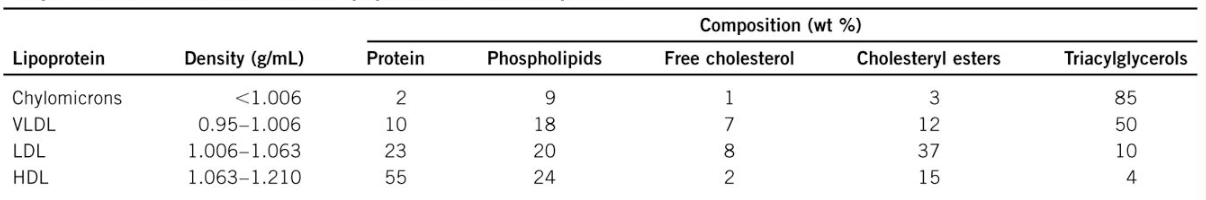
\includegraphics[width=0.8\textwidth]{fig30}
\label{fig30}
\end{figure}

La gravetat de les malalties s'ordenaria S�ndrome de Pearson > KSS > PEO.

\subsubsection{Malalties per mutaci� puntual}
\label{sec:malalt-per-mutac}

\begin{itemize}
\item MELAS (\textit{Myiopathy, stroke-like episodies, lactic acidosis}), degut a lesions focals al cervell al l�bul parito-occipital, acidosi l�ctica i/o RFFs.

\item MERRF (\textit{myoclonic epiplepsy}). Es troba \textit{red ragged fibers} a les fibres musculars. Mioclonus, epil�psia, debilitat muscular i RFF, at�xia cerebel�lar, sordesa i dem�ncia.

\item  NARP \textit{neuropatia, at�xia i retinitis pigmentosa}: Mutaci� puntual a ATP6. At�xia, retinopatia pigment�ria, neuropatia perif�rica i debilitat neurog�nica distal.

\item Hearing loss-ataxia-myoclonus: P�rdua d'o�da sindr�mica, epil�psia miocl�nica, at�xia, miopatia.

\item LHON: P�rdua de visi� central, escotoma gran absolut centrocecal gran, telangiect�sia circumpapil�lar, microangiopatia. LHON �s d'her�ncia materna (abans moltes malalties apareixien \textit{de novo}). Afecta el nervi �ptic. Diferents mutacions causals que afecten els gens ND (complex I de la cadena respirat�ria) al nervi �ptic. La c�l�lula t� adaptacions per viure sense NS.
\end{itemize}

\begin{figure}[H]
\centering
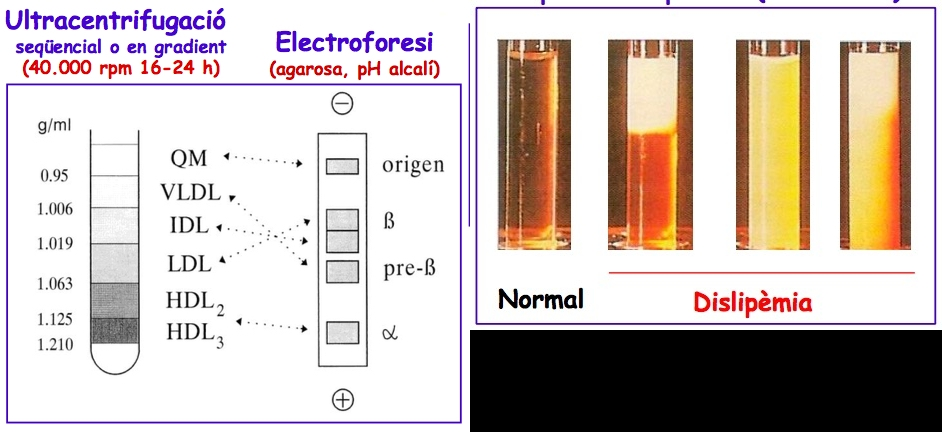
\includegraphics[width=0.8\textwidth]{fig31}
\label{fig31}
\end{figure}

Quan el m�scul es tenyeix amb tricr�mica de Gomori, apareixen fibres vermelles esquin�ades (RRF, \textit{red ragged fibers}) caracter�stiques que s�n visibles al microscopi. Aquest aspecte �s causa de l'acumulaci� dels mitocondris anormals per sota de la membrana plasm�tica de la fibra muscular. Aquests es poden estendre al llarg de la fibra muscular a mesura que augmenta la gravetat de la malaltia. Els agregats mitocondrials causen el contorn de la fibra muscular per convertir-se en irregular, provocant l'aparici� "desigual". A m�s dels m�sculs, el que altres teixits es pot esperar a patir m�s danys causats per un defecte mitocondrial?

La s�ndrome de Lay provoca apoptosi al cervell (encefalopatia necrotitzant). Tenen una mutaci� a ATP6 i m�s heteropl�smia que NARP.

Hi ha altres malalties causades per gens nuclears implicats en el manteniment del DNA mitocondrial i la cadena respirat�ria, com:
\begin{itemize}
\item Gens nuclears que codifiquen complexes de la cadena respirat�ria
\item Gens nuclears que codifiquen prote�nes implicades en l'estructura i assemblatge de complexes de la cadena respirat�ria
\item Gens nuclears que codifiquen prote�nes implicades en la replicaci� i transcripci� del DNA mitocondrial
\end{itemize}

\subsubsection{Deplecions}
La s�ndrome de depleci� del DNA mitocondrial (MDS) es refereix a un grup de trastorns autos�mics recessius que causen que els teixits afectats pateixin d'una depleci� significativa en el DNA mitocondrial. Els s�mptomes poden manifestar-se com miop�tics, hepatop�tics, i/o encefalomiop�tics. Aquests s�ndromes afecten teixits que es troben en el m�scul, el fetge, o tant el m�scul i el cervell, respectivament. La condici� sol ser mortal en la inf�ncia i la infantesa primerenca, encara que alguns han sobreviscut als seus anys d'adolesc�ncia amb la variant miop�tics i alguns han sobreviscut fins a l'edat adulta amb la variant encefalomiop�tica SUCLA2. Actualment no existeix un tractament curatiu per a qualsevol forma de MDS.

Les caracter�stiques de la depleci� s�n:
\begin{itemize}
\item Disminuci� de les c�pies de DNA

\item Her�ncia autos�mica recessiva

\item Gran heterogene�tat cl�nica

\item Associaci� amb mutacions en molts gens: TK2, DGUOK, MPV17, POLG1, C10ORF2, SUCLA2, 	SUCLG1, RRM2B, TYMP.
\end{itemize}

\begin{figure}[H]
\centering
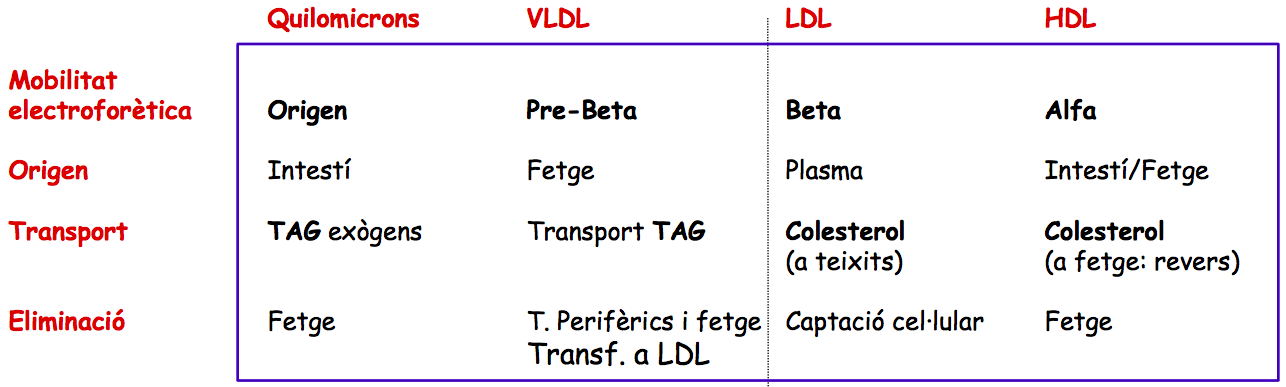
\includegraphics[width=1\textwidth]{fig32}
\label{fig32}
\end{figure}

La forma miop�tica de MDS manifesta s�mptomes dins el primer any de vida, i es diagnostica per la pres�ncia de nivells m�s alts de s�rum de CK, que �s at�pic en altres miopaties mitocondrials. El MDS miop�tic est� fortament correlacionat amb mutacions en el gen TK2, en veure una reducci� de l'activitat TK2 a menys del 32\% en pacients amb MDS trobats amb la mutaci�. Donat que el TK2 juga un paper clau en les rutes de recicaltge mitocondrials de diversos dNTPs, una activitat rebaixada conduiria a menys reciclatge de nucle�tids. Aquesta manca de reciclatge de nucle�tids �s perjudicial ja que els mitocondris no poden sintetitzar completament nous dNTP, i la membrana interna del mitocondri evita que entrin els nucle�tids carregats negativament del citosol. Hi ha una gran variabilitat en el grau de depleci� del mtDNA als teixits afectats, entre el 66 i el 86\%. Es troben RRF al m�scul esquel�tic i defici�ncies en cadenes respirat�ries. Els aspeces cl�nics s�n hipotonia forta, acidosi l�ctica, oftalmopl�gia, lordosi lumbar i dipl�gia facial.

\begin{figure}[H]
\centering
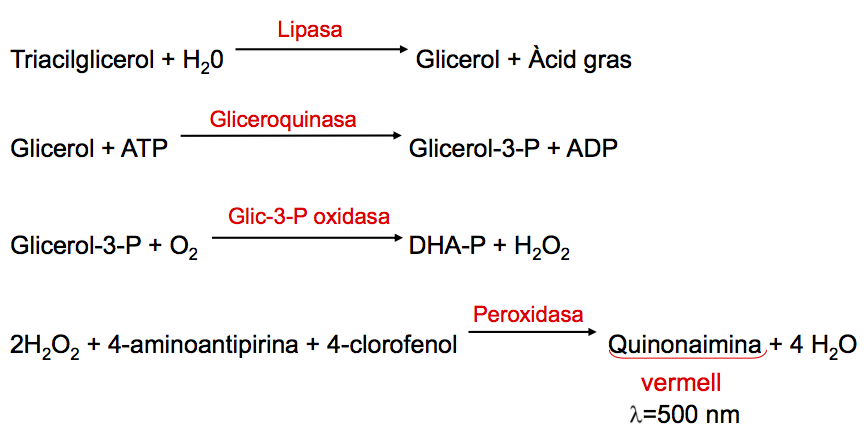
\includegraphics[width=0.8\textwidth]{fig34}
\label{fig34}
\end{figure}

La forma encefalomiop�tica de MDS es caracteritza comunament per retard psicomotor, hipotonia muscular, p�rdua d'audici�, i convulsions generalitzades. Una mutaci� comuna en aquesta forma de MDS �s en el gen SUCLA2, que codifica per a la subunitat $\beta$ de SCS-A. Aquest enzim catalitza la s�ntesi de succinat i coenzim A en succinil-CoA, per� tamb� s'associa amb el complex format per nucle�sid difosfat quinasa (NDPK) en l'�ltim pas de la via de reciclatge de dNTP. Altres formes s'han associat amb mutacions en el gen RRM2B.

La forma hepatop�tiques de MDS consisteixen en l'aparici� de s�mptomes que inclouen hipotonia, hipogluc�mia, v�mits persistents, i la falta de creixement durant el primer any de vida. Les mutacions en tres gens s'han relacionat amb MDS hepatop�tiques : DGUOK, POLG, i Mpv17. DGUOK codifica per la desoxiguanosina cinasa mitocondrial (DGK), que catalitza la fosforilaci� de desoxirribonucle�sids en nucle�tids. POLG codifica per a la subunitat catal�tica $\gamma$A pol, que �s part de la polimerasa de DNA mitocondrial. En aquest cas, la malaltia comen�a en una edat primerenca, t� un mal pron�stic i �s letal durant els primers mesos de vida. La depleci� de mtDNA als teixits afectats �s molt severa (88-99\%) i la defici�ncia de la cadena respirat�ria �s molt greu. Cl�nicament es manifesta com a insufici�ncia hep�tica progressiva, complicacions neurol�giques, hipoglic�mia, hiperlactat�mia.

\begin{figure}[H]
\centering
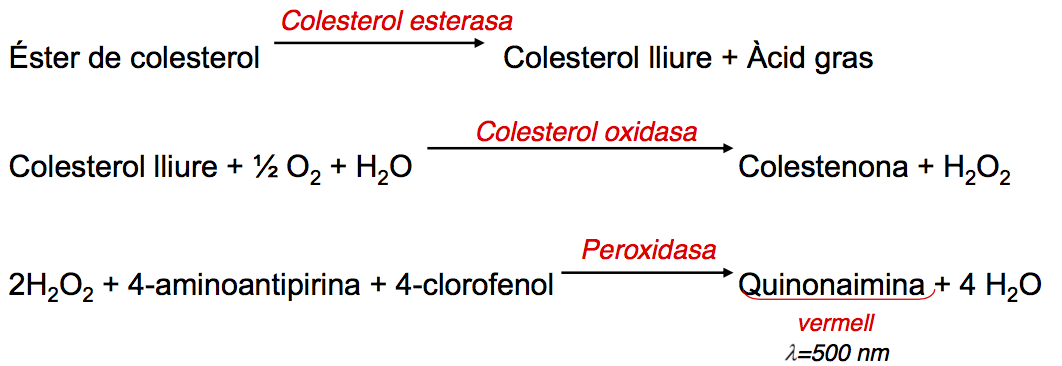
\includegraphics[width=0.8\textwidth]{fig33}
\label{fig33}
\caption{Associaci� entre gens de s�ndrome de depleci� mitocondrial i teixits afectats}
\end{figure}

Algunes MDS s'associen amb mutacions som�tiques al mtDNA, com el MNGIE (\textit{Mitochondrial neurogastrointestinal encephalopathy syndrom}).

La s�ndrome d'encefalopatia neurogastrointestinal mitocondrial (MNGIE) �s un trastorn gen�tic autos�mic recessiu poc freq�ent que generalment apareix entre la segona i la cinquena d�cada de la vida. A difer�ncia de les usuals malalties mitocondrials, que s�n causades per mutacions en l'DNA mitocondrial (DNAmt), la MNGIE �s causada per mutacions en el gen TYMP (localitzat al cromosoma 22q13.32), el qual �s codificat per l'anomenat enzim timidina fosforilasa. Una de les formes secund�ries d'aquesta s�ndrome s'anomena MNGIE sense leucoencefalopatia i pot �sser causada per mutacions en el gen POLG.

Al voltant de 50 mutacions en el gen TYMP han estat identificades en persones amb la s�ndrome de MNGIE. Les mutacions en el TYMP redueixen notablement o eliminen l'activitat de la timidina fosforilasa. L'escassetat d'aquest enzim permet que la timidina s'acumuli al cos en grans quantitats i un exc�s d'aquest subst�ncia �s perjudicial per al DNAmt, ja que altera el seu funcionament habitual (manteniment i reparaci�). Conseg�entment, les mutacions es poden anar acumulant a l'interior del DNAmt causant-li inestabilitat i tamb� pot ser que els mitocondris continguin menys DNAmt de l'habitual. Tots aquests canvis gen�tics alteren el funcionament mitocondrial normal. Malgrat saber que les anomalies del DNAmt emmarquen els problemes digestius i neurol�gics caracter�stics de la s�ndrome MNGIE, avui en dia encara es desconeix com el mitocondri defectu�s causa els trets caracter�stics espec�fics propis de la malaltia.

La MNGIE �s un trastorn autos�mic recessiu (�s a dir, no est� lligada al sexe i per tal que es manifesti cal heretar els dos al�lels mutants), per tant els progenitors han de ser com a m�nim portadors de l'al�lel mutant; els heterozigots no presenten cap s�mptoma. Els medicaments que interfereixen amb la funci� mitocondrial s'han d'evitar tant com sigui possible i utilitzar amb precauci� aquells que es metabolitzin al fetge.

\subsection{Tractament de les malalties mitocondrials}
\label{sec:tractament-de-les}
Hi ha diferents estrat�gies:
\begin{itemize}
\item \textbf{Ter�pia pal�liativa:} Inclou f�rmacs anticonvulsius, control de les alteracions endocrines i procediments quir�rgics.

\item \textbf{Eliminaci� de metab�lits nocius:} Principalment el lactat de l'acidosi l�ctica, per� tamb� timidina en pacients MNGIE.

\item \textbf{Administraci� d'acceptors d'electrons:} Per evitar alguns components de la cadena respirat�ria.

\item \textbf{Administraci� de metab�lits i cofactors:} �s la base de la ter�pia actual. Inclou components de la cadena respirat�ria i altres com L-carnitina o CoQ10 (ubiquinona).

\item \textbf{Scavengers de ROS:} Tant en malalties mitocondrials prim�ries com en malalties neurodegeneratives causades directa o indirectament per una disfunci� mitocondrial.
\end{itemize}

Hi ha estrat�gies de FIV per trasplantar els mitocondris d'una donant sana:
\begin{figure}[H]
\centering
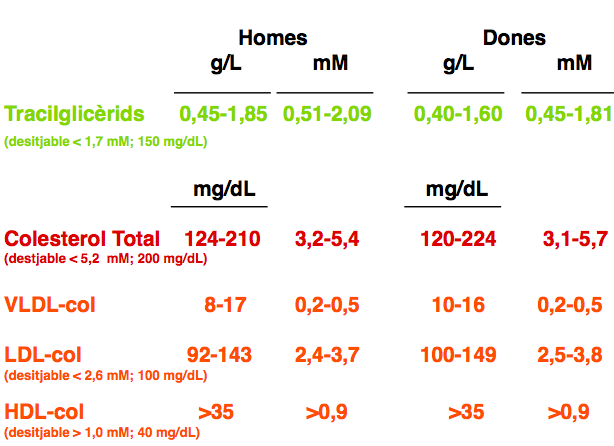
\includegraphics[width=0.8\textwidth]{fig35}
\label{fig35}
\end{figure}

El tractament amb antiretrovirals causa una depleci� del mtDNA, el que acaba en una lipodistr�fia adquirida en pacients amb SIDA. La lipodistr�fia adquirida es caracteritza per una p�rdua severa de teixit adip�s perif�ric per� amb una adipositat central. Els pacients tenen hipertriglicerid�mia, hipercolesterol�mia, acidosi l�ctica, resist�ncia a la insulina i diabetis de tipus 2. Es creu que �s degut a que els an�legs de nucle�sids usats pel tractament del VIH inhibeixen la DNA polimerasa mitocondrial.

%------------------------------------------------------------------------------
% Tema 5. Hemost�sia i coagulaci�
%------------------------------------------------------------------------------
%\newpage
%%------------------------------------------------------------------------------
% Tema 5. Genètica de la obesitat
%------------------------------------------------------------------------------
\section{Genètica de la obesitat monogènica}
\label{sec:genetica-de-la}

\subsection{Obesitat monogènica}
\label{subsec:obesitat-monogenica}
Les nenes deficients en leptina tenen problemes de maduració sexual i per tant de fertilitat.

Els pacients deficients en MC4R (receptor de melanocortina), que són heterozigots per la mutació. Presenta obesitat a la infància, hiperfàgia, hiperinsulinèmia.

Hi ha 2 tipus de pèptids que controlen la sacietat quan senyalitzen a l'hipotàlem:
\begin{itemize}
\item Orexigènics Inhibits per la leptina
\item Anorexigènics: Estimulats per la leptina. El gen de la POMC quan s'expressa genera un polipèptid de 31 kDa, que en funció de les cèl·lules on s'expressa la proteïna es trenca en diferents fragments que seran els que tenen l'activitat biològica. Aquests fragments poden ser la ACTH, alpha-MSH... alpha-MSH atura la gana, interaccionant amb un receptor hipotalàmic. Quan el nen té dèficits en POMC, es poden donar agonistes pel receptor hipotalàmic.
\end{itemize}

\subsection{Obesitat multifactorial}
\label{subsec:obes-mult}

% tipus d'estudi per identificar gens de susceptibilitat

El gen FTO té una variant que s'associa molt potentment a un BMI alt. En canvi, variants polimòrfiques de la leptina no tenen associació amb la obesitat. BDNF fa de connexió entre l'hipotàlem i l'escorça per generar la sensació conscient de gana/sacietat.

FTO se sabia que tenia un NLS, un domini de demetilasa. FTO es troba en una regió genòmica amb clústers d'IRX (iroguis-related). Introns del FTO regulen els enhancers del gen IRX; el grau d'interacció condiciona l'expressió d'IRX3. IRX3 re demetilasagula la despesa energètica. Els al·lels FTO de risc per obesitat que quan interaccionen amb IRX3 augmenten l'expressió d'IRX3, i IRX3 disminueix la despesa energètica.

%------------------------------------------------------------------------------
% Tema 6. Hemoglobina i ferro
%------------------------------------------------------------------------------
\newpage
%------------------------------------------------------------------------------
% Tema 6. Hemoglobina i ferro
%------------------------------------------------------------------------------
\section{Hemoglobina i ferro}

\subsection{La hemoglobina}
La hemoglobina �s una prote�na globular que dona la coloraci� vermella
de la sang. Responsable del transport de \ch{O2}. T� un pes de  64,45
kDa.

Els nivells normals s�n de 16g/100 mL en homes i de 14g/100 mL en les dones.

Un home de 70 kg t� 900 g d'hemoglobina. El bescanvi d'hemoglobina �s
de 0,3 g/h (sintetitzats i destru�ts).

Classificaci� de les malalties relacionades amb la hemoglobina:
\begin{itemize}
\item Reaccions de l'hemoglobina
  \begin{itemize}
  \item Metahemoglobin�mia heredit�ria
  \end{itemize}

\item S�ntesi de la globina
  \begin{itemize}
  \item Hemoglobinopaties estructurals
    \begin{itemize}
    \item An�mies drepanoc�tiques 
    \item Metahemoglobin�mia cong�nita
    \item Eritrocitosis (alterada afinitat per O2)
    \end{itemize}
  \item Talass�mies (hemoglobines alterades)
    \begin{itemize}
    \item  $\alpha$-talass�mies
    \item $\beta$-talass�mies
    \end{itemize}
  \end{itemize}

\item S�ntesi i degradaci� del grup hemo
  \begin{itemize}
  \item Porfiries agudes
    \begin{itemize}
    \item Porf�ria aguda intermitent 
    \item Coproporf�ria heredit�ria
    \item Porf�ria variegata
   \end{itemize}
  \item Porf�ries no agudes
    \begin{itemize}
    \item Porf�ria eritrohep�tica (eritropoi�tica) 
    \item Porf�ria eritropoi�tica cong�nita
    \item Porf�ria cong�nita (Intoxicaci� per plom)
    \end{itemize}
  \end{itemize}

\item Alteracions del metabolisme del ferro
  \begin{itemize}
  \item An�mia ferrop�nica (manca de ferro)
    \begin{itemize}
    \item P�rdua cr�nica de sang
    \item Ingesta inadequada de ferro
    \end{itemize}
  \item An�mia siderobl�stica (mala utilitzaci� del ferro)
  \item Hemocromatosis (sobrec�rrega de ferro)
  \end{itemize}
\end{itemize}

\subsubsection{Estructura}
Hi ha 6 tipus de globines, que en la seva combinat�ria generen els
diferents tipus d'hemoglobina que trobem en humans. Aquests tipus s�n:
$\alpha$, $\beta$, $\gamma$, $\delta$, $\epsilon$, $\zeta$.

La hemoglobina �s un heterotetr�mer $\alpha_2\beta_2$ en adults. Presenta
cooperativitat amb l'oxigen. Tamb� t� al�losterisme amb el
2,3-difosfoglicerat, un intermediari de la glic�lisi que nom�s es
troba en eritr�cits. Aix� facilita l'alliberaci� d'oxigen als
teixits.

Es sintetitza als reticul�cits (eritr�cits immadurs).

La hemoglobina presenta diferents subunitats segons l'estadi de
desenvolupament de l'individu:
\begin{itemize}
\item Adult:
  \begin{itemize}
  \item Hemoglobina A1 ($\alpha_2\beta_2$)
  \item Hemoglobina A2 ($\alpha_2\delta_2$)
  \end{itemize}

\item Fetal: Cadenes $\alpha_2\gamma_2$

\item Embri�:
  \begin{itemize}
  \item Grower I: $\zeta_2\epsilon_2$
  \item Grower II: $\alpha_2\epsilon_2$
  \item Portland: $\zeta_2\gamma_2$
  \end{itemize}
\end{itemize}

Hi ha 2 loci d' $\alpha$-globina al cromosoma 16 i un locus de $\beta$-globina
al cromosoma 11.

\subsection{Trastorns deguts a reaccions de l'hemoglobina}
La carboxihemoglobina presenta menys afinitat per l'hemoglobina.

\begin{figure}[H]
  \centering
  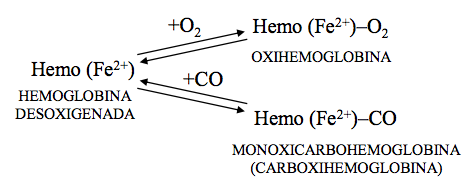
\includegraphics[width=0.5\textwidth]{fig5}
\end{figure}

Molt f�rmacs o agents oxidants poden provocar la formaci� de
metahemoglobina (amb \ch{Fe3+}), que mitjan�ant la NADH-metahemoglobina
reductasa la torna a reduir.

\begin{figure}[H]
  \centering
  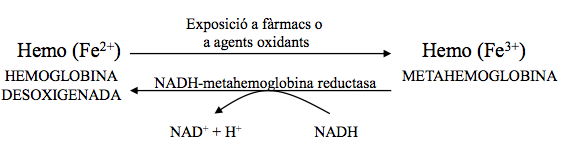
\includegraphics[width=0.5\textwidth]{fig6}
\end{figure}

La metahemoglobin�mia heredit�ria �s una defici�ncia en NADH-metahemoglobina
reductasa. El Fe del hemo s'oxida en 25 \% a \ch{Fe3+} Es manifesta amb
cianosi (coloraci� fosca a la pell). Es tracta amb f�rmacs que
redueixin lametahemoglobina. �s una malaltia
molt greu.

\subsection{Trastorns a la s�ntesi de la globina}
\subsubsection{Hemoglobinopaties estructurals}
Les mutacions perjudicials desapareixen, per� les altres poden sobreviure
(els heterozigots resisteixen m�s que els homozigots). Algunes
mutacions s�n in�cues.

\paragraph{Hemoglobina S. An�mia drepanoc�tica} \hfill \\
Es d�na un canvi d'amino�cid Glu->Val a la cadena beta. �s insoluble a baixes pressions
de \ch{O2}. Els gl�buls vermells presenten una morfologia
falciforme. Quan est� desoxigenada, la hemoglobina es polimeritza i es
deformen els eritr�cits. Els heterozigots  presenten poques vegades s�mptomes greus

Es va originar a Africa i confereix resist�ncia a la mal�ria. La
presenten un 40 \% de la poblaci� africana i un 10\% dels negres
americans.

La Hb pot polimeritzar formant fibres de 3000 \AA{}. Hi ha cicles
successius de forma de fal� i normal. La forma de fal� es trenca als
capil�lars per falta de flexibilitat. L'an�mia s'agreuja amb oxidants.

Altes concentracions d'HbS d'afinitat baixa per \ch{O2} no donen cap
problema fins l'administraci� d'un agent oxidant.

L'an�mia �s menys severa si �s dependent d'HbF. Els pacients tendeixen
a augmentar la proporci� d'HbF en l'adult. Els homozigots d'Orient
Mitj� s�n asimptom�tics ja que tenen un 18\% d'HbF.

El diagn�stic es fa per electroforesi de la hemoglobina o per examen
microsc�pic d'un frotis de sang.

Encara no hi ha tractament, encara que hi ha f�rmcs en estudi. La
profilaxi es basa en una bona nutrici� i higiene, contra la
mal�ria. En cas d'infecci�, s'actua sobre l'agent infecci�s. Si es fa
una transfusi� quan es dona la primoquina ja que �s oxidant i es pot
agreujar l'an�mia.

\paragraph{Hemoglobinopaties inestables} \hfill \\
S'han descrit m�s de 100 hemoglobinopaties. Es produeix la formaci� de
cossos d'inclusi� intraeritroc�tics (cossos de Heinz), que s�n
precipitacions d'hemoglobina. Consisteix en una s�rie de petites
granulacions que se situen a la perif�ria dels hematies. Es produeix
en malalties cong�nites.

\begin{figure}[H]
  \centering
  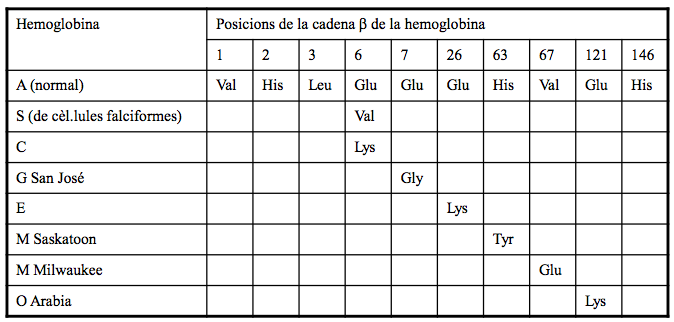
\includegraphics[width=0.8\textwidth]{fig7}
  \caption{Composici� parcial en amino�cids en la cadena $\beta$ humana
    normal i algunes hemoglobines amb cadenes $\beta$ anormals. Altres
    hemoglobines tenen cadenes $\alpha$ anormals.}
  \label{fig:fig7}
\end{figure}

\paragraph{Eritrocitosis} \hfill \\
Alteraci� en l'afinitat per \ch{O2}. En casos lleus no requereix
farmacologia. L'afinitat �s m�s alta degut a canvis que eviten la uni�
de 2,3-difosfoglicerat. Es produeix una hip�xia lleu (augment d'eritr�cits).

\subsubsection{Talass�mies}

%------------------------------------------------------------------------------
% Tema 7. Enzimologia cl�nica
%------------------------------------------------------------------------------
\newpage
%------------------------------------------------------------------------------
% Tema 7. Enzimologia cl�nica
%------------------------------------------------------------------------------
\section{Enzimologia cl�nica}

\subsection{Enzims}
L'enzimologia cl�nica �s un conjunt de t�cniques destinades a detectar
la pres�ncia i a quantificar l'activitat d'enzims en mostres biol�giques:
\begin{itemize}
\item Pres�ncia d'enzims que no es trobin normalement en
  concentracions significatives
\item Variacions en els nivells d'enzims que poden trobar-se
  normalment en mostres biol�giques
\item Isoenzims (formes diferents d'un enzim)
\end{itemize}

Es poden utilitzar enzims com a reactius espec�fics per quantificar la
concentraci� de metab�lits.

Un enzim �s un biocatalitzador proteic. Es localitzen en tots els
teixits corporals. Es determinen mitjan�ant la reacci� enzim�tica. Un
holoenzim est� format per un apoenzim (porci� proteica) i coenzim
(porci� no proteica no sempre necess�ria). L'activitat enzim�tica es
pot veure redu�da si no hi ha apoenzim o coenzim.

Els enzims tenen destrucci� citoplasm�tica o mitocondrial. A la
circulaci� es poden eliminar per catabolisme que alliberar� amino�cids
i grups prost�tics per la s�ntesi de noves prote�nes i/o enzims.

Tots els enzims s�rics tenen un origen cel�lular. Apareixen al s�rum
com a conseq��ncia d'una lesi� cel�lular (en petites quantitats de la
degradaci� cel�lular). Les activitats enzim�tiques del s�rum s�n �tils
pel diagn�stic de malalties particulars o anomalies fisiol�giques.

Quan les c�l�lules estan en proliferaci�, augmenta la s�ntesi d'enzims
i s'atura el seu catabolsime. En l'estat d'inactivaci�, hi ha un
descens de la s�ntesi d'enzims i augmenta la seva degradaci� degut a
la car�ncia de cofactors. 

Els enzims difonen a la limfa, passen a la sang on s'inactiven (p�rdua
de grups prost�tics, canvis conformacionals) i es catabolitzen. Els
enzims es destrueixen en fag�cits, melsa, endotelials, c�l�lules sangu�nies.

L'�s de certs enzims per diagnosticar malalties �s per circumst�ncies
hist�riques. No �s normal que un enzim que funciona sigui substitu�t
per un altre, a no ser que la utilitat diagn�stica sigui molt millor.

\subsubsection{Lesi� cel�lular}
Hi ha enzims i metab�lits intracel�lulars i extracel�lulars en una
situaci� normal. Si hi ha una lesi� cel�lular, es detecten enzims i
metab�lits intracel�lulars a la sang.

Els enzims intracel�lulars poden apar�ixer al plasma degut als
processos normals de recanvi cel�lular. L'increment dels enzims pot
ser degut a la lesi� cel�lular o a l'augment de la proliferaci�.

\subsubsection{Mesura de la concentraci� dels enzims}
\begin{itemize}
\item \textbf{Concentraci� de massa:} Quantitat de l'enzim.
\item \textbf{Concentraci� catal�tica:} Activitat de l'enzim. �s el
  m�s usat. Es pot expressar com a:
  \begin{itemize}
  \item Activitat enzim�tica: Quantitat d'enzim que transforma un
    micromol de substrat per minut a 25�C. Es poden fer servir UI o katals.
  \item Activitat espec�fica: Unitats de l'enzim per mil�ligram de prote�na
  \item Activitat molecular o molar: N�mero de mol�cules de substrat
    trasformades per minut per
una sola mol�cula d'enzim
  \end{itemize}
\item Concentraci� d'isoformes: Permet discriminar el teixit d'origen.
\end{itemize}

L'activitat enzim�tica pot variar degut a la temperatura, pH,
concentraci� de substrat, for�a i�nica... La prova s'ha d'adequar a
les concentracions �ptimes de l'enzim.

\subsubsection{Distribuci� cel�lular dels enzims}
% Taula
\begin{table}[H]
  \centering
  
  \caption{Localitzaci� subcel�lular d'enzims amb import�ncia cl�nica}
  \label{tab:enzims}
\end{table}

La pres�ncia d'enzims mitocondrials en s�rum �s indicatiu de dany greu.

La detecci� d'una isoforma permet fer un diagn�stic m�s prec�s. Es
poden detectar per:
\begin{itemize}
\item Difer�ncia de c�rrega neta (cromatografia, electroforesi,
  isoelectroenfocament)
\item Acci� selectiva de determinades subst�ncies (inhibici�
  selectiva)
\item T�cniques immunol�giques (immunoinhibici�, enzimimmunoassaig)
\end{itemize}

Poden alliberar-se els enzims encara que no hi hagi necrosi h�stica
(augment de la permeabilitat de les membranes) als teixits. Exemple:
delirium tremens.

La fosfatasa alcalina �s un marcador per malalties hepatobiliars. En
canvi, hi ha altres enzims m�s bons com la leucinaminopeptidasa o la
5'-nucleotidasa.

Un altre exemple �s la GPT (hepatopatia) que no ha estat substitu�da
per la ornitin-carbamo�l-transferasa o iditol-deshidrogenasa.

\subsubsection{Inter�s diagn�stic dels enzims}
Les an�lisis enzim�tiques representen fins un 20\% de les proves
bioqu�miques. Els laboratoris de bioqu�mica cl�nica poden determinar
entre 12-15 enzims diferents.

Actualment s'han determinat me??s de 60 enzims en s�rum, dels quals:
\begin{itemize}
\item Alguns es determinen habitualment al laboratori
\item Alguns s�n reflex de diverses malalties, per� no es determinen
  degut a la seva dificultat
\item Alguns s�n importants a nivell de recerca, i nom�s es determinen
  en situacions cl�niques especials
\end{itemize}

% posar taula

\subsection{Estrat�gies bioqu�miques per l'estudi cl�nic del
  metabolisme}

Els enzims es poden estudiar de diferents maneres:
\begin{enumerate}
\item Determinaci� de la concentraci� de metab�lits en l�quids i
  teixits biol�gics
\item Determinaci� d'activitats enzim�tiques en l�quids i teixits
  biol�gics
\item Diferenciaci� de les formes isoenzim�tiques
\item An�lisi de la resposta metab�lica en front proves diagn�stiques
  espec�fiques
\end{enumerate}

\subsubsection{Cin�tica de les reaccions enzim�tiques monosubstrat}
Si:
\begin{itemize}
\item L'espectrofot�metre absorbeix el substrat, l'absorb�ncia
  disminuir� en funci� del temps.
\item L'espectrofot�metre absorbeix el producte, l'absorb�ncia
  augmentar� en funci� del temps.
\end{itemize}

S'ha d'escollir la longitud d'ona on es distingeixi l'absorci� del
substracte de la del producte.

\subsubsection{Procediments per a mesurar la velocitat de
  transformacio??}

Hi ha 2 tipus:
\begin{enumerate}
\item \textbf{Procediments discontinus:}
  \begin{enumerate}
  \item A un punt.- Es mesura l???absorba??ncia de la mostra i de un blanc
    al cap d???un temps determinat.
    \begin{equation}
      \label{eq:1}
      v = \frac{A_t-A_{Blanc}}{t}
    \end{equation}
  \item A dos punts.- Es mesuren 2 absorba??ncies (A1, A2) a dos temps
    (t1, t2).
    \begin{equation}
      \label{eq:2}
      v = \frac{A_2-A_1}{t_2-t_1}
    \end{equation}
  \item A tres o me??s punts.- Es mesura l???absorba??ncia a diversos valors
    de temps (mesurar dos punts pot ser inexacte).
    \begin{equation}
      \label{eq:3}
      v = \frac{\Delta A}{\Delta t}
    \end{equation}
  \end{enumerate}

\item \textbf{Procediments continus:} Es mesura l???absorba??ncia
  continuament durant un temps determinat.
  \begin{equation}
    \label{eq:4}
    v = \frac{d A}{d t} 
  \end{equation}
\end{enumerate}

\subsubsection{Aplicacio?? de te??cniques enzima??tiques combinades}
La concentraci� dels enzims �s molt baixa (nmol) i per tant es mesura
la seva activitat (o b� s'aplica immunoan�lisi).

Hi ha 3 fases de l'activitat enzim�tica:
\begin{enumerate}
\item Periode de lante??ncia. La velocitat va augmentant progressivament.
\item Estat estacionari. La velocitat e??s proporcional a la
  concentracio?? de l???enzim. 
\item Fase final.- la velocitat disminueix progressivament e??s on es fa
  l'an�lisi)
\end{enumerate}

La malalt deshidrogenasa t� concentracions molt baixes, per tant
s'aplica a reaccions acoblades. Es mira l'activitat de l'enzim
anterior o posterior.

% Exemple de diap 13.

\subsubsection{Procediment general d'an�lisi per espectrofotometria
  visible o UV}
L'espectrosc�pia estudia els sistemes mitjan�ant la seva interacci�
amb les radiacions electromagn�tiques. Un sistema �s un conjunt de
part�cules materials (�toms, mol�cules).
\begin{itemize}
\item Absorci�
\item Emissi�
\item Difracci�
\end{itemize}

L'espectrometria d'absorci� molecular UV-visible �s molt utilitzada en
cl�nica. Estudia l'absorci� de la radiaci� magn�tica ultravioleta i
visible. Permet mesurar la concentraci� d'una subst�ncia.

L'espectre electromagn�tic �s el conjunt de totes les longituds d'ona.

En un laboratori cl�nic s'utilitza amb m�s freq��ncia les regions
visible i ultraviolada.

Els espectrofot�metres poden ser de:
\begin{itemize}
\item Feix simple: Primer es posa el blanc com a refer�ncia i despr�s
  la mostra.
\item Feix doble: Detecta el blanc i la mostra alhora.
\end{itemize}

\subsection{Enzims marcadors habituals en enzimologia cl�nica}


%=================================================================
%=================================================================
\newpage
\phantomsection
\addcontentsline{toc}{part}{Refer�ncies}
\begin{multicols}{2}
\bibliography{bibbac} 
\bibliographystyle{authordate3}
\end{multicols}

\end{document}

Els de BIOMED fem un parcial. Val un 10\% extra.

El final �s 60 preguntes tipus test, 3 preguntes curtes de cada part +
10 preguntes de pr�ctiques.

Treball: Vicent Casad�